\subsection{Flight screens}\label{subsec:flight-screens}
The \textbf{Flights screen} (Figure \ref{fig:flights}) is for displaying a list of the flights.
This screen contains flight statistics and allows finding certain flights by chosen filters.
By every flight, it shows its state if it is planned and current flight.
Besides, it contains the button for exporting the whole flight history.
If a user chooses a planned flight, it shows the Flight plan screen, which is a planned flight summary and consists of various parameters.
It is possible to show the \textbf{Flight detail} screen for finished flights, and the \textbf{In-flight detail} screen for current flights.

The \textbf{Flight detail screen} contains all information about a flight, including the option to play flight track from start to the end.
The \textbf{In-flight detail screen} contains information about the flight in real-time.
Thanks to the \textbf{Sliding up panel} we can see more information and still check if a drone did not escape the reservation area.

The \textbf{Plan a flight} is a group of three screens that represent a wizard for flight plan.
In the first screen, the user sets identification properties and planned time of flight.
In the second screen, the user sets a polygon for planned flight and its maximum altitude.
In the last screen, the user confirms set parameters of planned flight - it is like a summary.


\begin{figure}
    \centering
    \begin{minipage}{.4\textwidth}
        \centering
        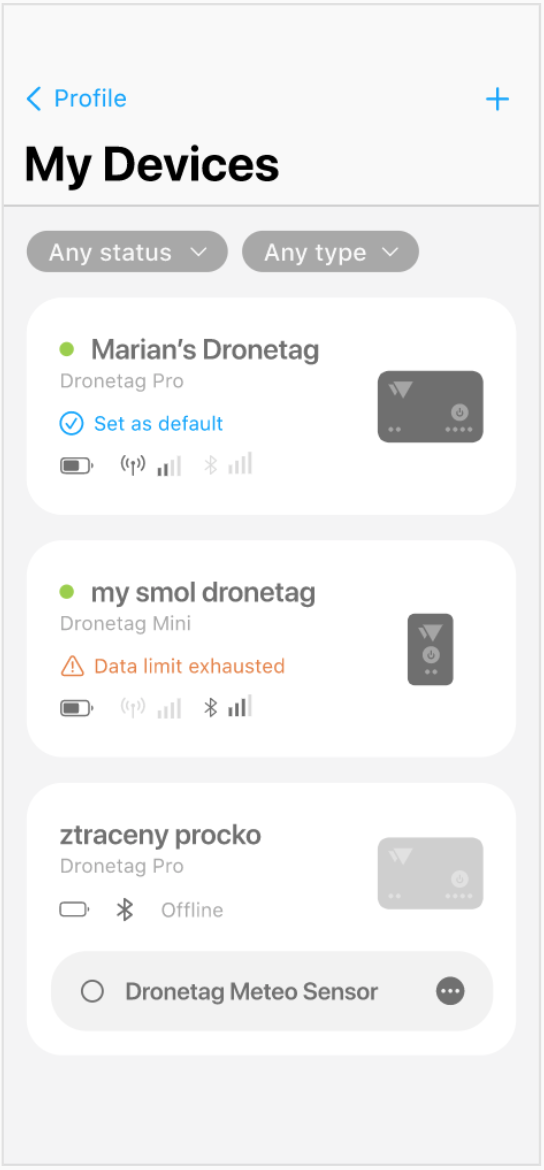
\includegraphics[width=.7\linewidth]{assets/user_interface_design/device/devices.png}
        \caption{Devices}
        \label{fig:devices}
    \end{minipage}%
    \hspace{.05\linewidth}
    \begin{minipage}{.4\textwidth}
        \centering
        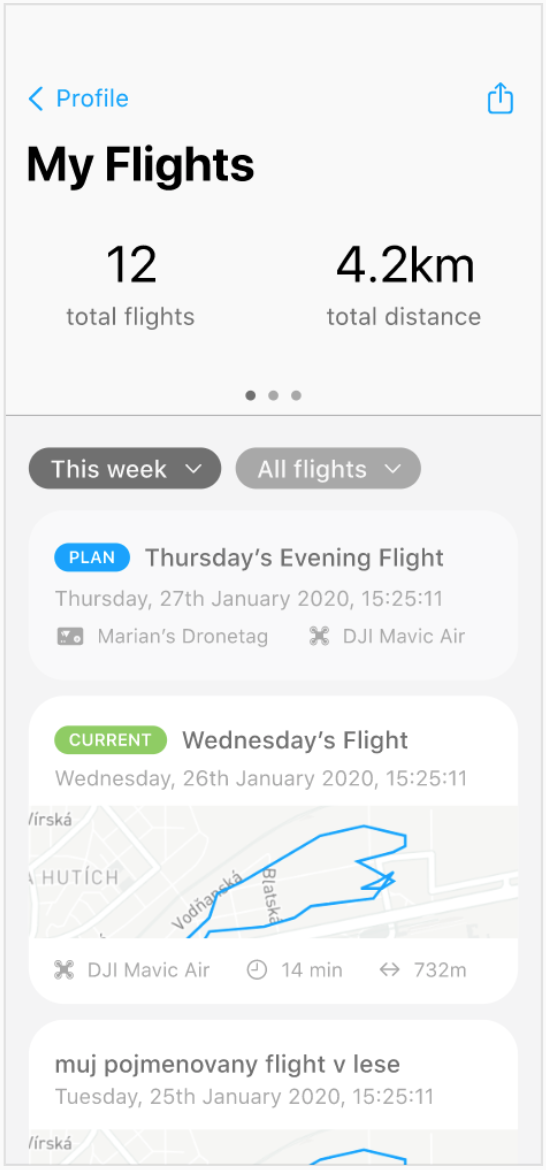
\includegraphics[width=.7\linewidth]{assets/user_interface_design/flight/flights.png}
        \caption{Flights}
        \label{fig:flights}
    \end{minipage}%
    \label{fig:flight_all}
\end{figure}
